Das Logo der App dient als Splashscreen (Abbildung \ref{fig:splashundmenu}). Nach dem Laden wird man von der Home-Seite begrüsst. Streift man mit dem Finger von Links nach Rechts oder klickt auf das Menü-Sandwich, öffnet sich ein Side-Menü. Das Side-Menü hat oben wieder das Logo und darunter zwei Texte ("`Magic 2 Brain"' und "`Your MTG learning companion"'). Unter dem befinden sich 7 Schaltflächen mit den Texten: "`Home"', "`Search"', "`Set Browser"', "`Quick Learn"', "`Favorites"', "`Recently Learned"' und "`Share"' (Abbildung \ref{fig:splashundmenu}).

\begin{figure}[htbp]
 \centering
    
\includegraphics[width=0.3\textwidth]{startup.jpg}
    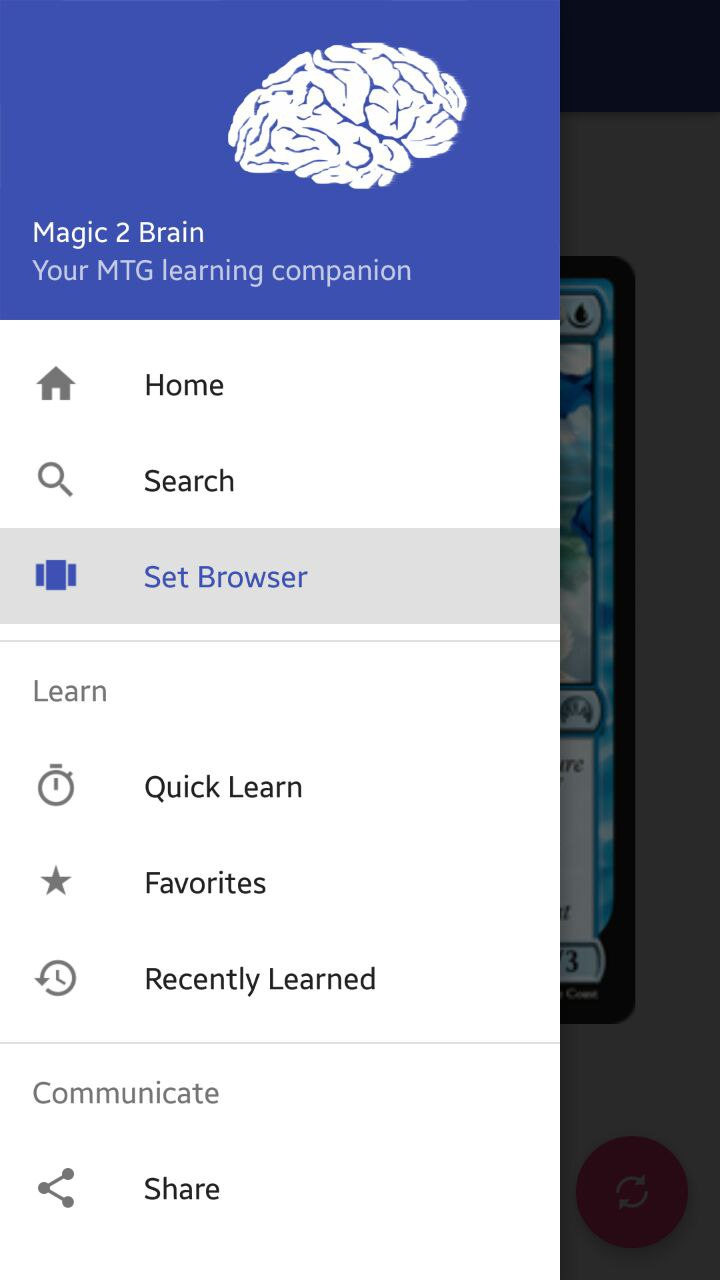
\includegraphics[width=0.3\textwidth]{sidemenu.jpg}
 \caption{Links: Der Splash-Screen, Rechts: Das Menü}
 \label{fig:splashundmenu}
\end{figure}

\subsection{Home}
Der Homescreen ist simpel aufgebaut. Ganz oben ist "`Magic2Brain"' geschrieben und direkt unter dem "`Random Card"'. Mitten auf dem Bildschirm ist eine zufällige Karte abgebildet. Mit einem Klick auf die Karte lässt sich diese vergrössern. Ganz unten rechts ist ein runder Knopf. Dieser ersetzt bei einem Klick die Karte mit einer anderen zufälligen Karte. (Abbildung \ref{fig:homemenu}).

\begin{figure}[htbp]
 \centering
    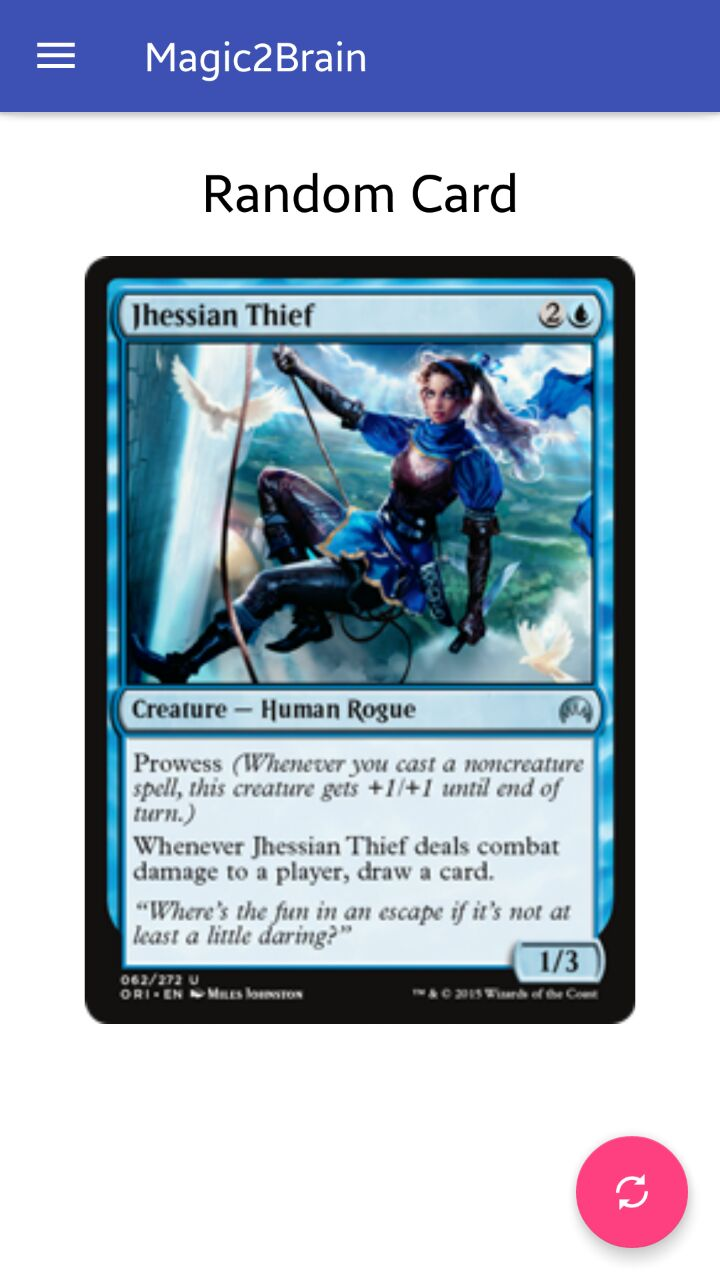
\includegraphics[width=0.3\textwidth]{home.jpg}
 \caption{Der Home-Screen \cite{Magiccard}}
 \label{fig:homemenu}
\end{figure}

\subsection{Search}
Wird auf "`Search"' gedrückt, kann ausgewählt werden, ob nach Karten oder Sets gesucht wird. Wählt man eine der beiden Optionen aus, wird man zu einer Ansicht mit einem Textfeld über einer Liste weitergeleitet. Tippt man etwas in das Textfeld ein, ändert sich die Liste und zeigt nur die Suchergebnisse an.

\subsection{Set Browser}
Der Set-Browser zeigt alle Sets in einer Liste an (Abbildung \ref{fig:setbrowser}). Drückt man auf ein Set, erscheint eine weitere Ansicht mit einer Liste. Diese Liste beinhaltet alle Karten vom ausgewählten Set. Navigiert man auf eine Karte, sieht man die Karte in einer Detailansicht. Bild, Text, Manakosten und der Name der Karte werden angezeigt (Abbildung \ref{fig:setbrowser}). Zudem hat man einen Knopf mit einem Herzen drauf. Betätigt man diesen, wird die Karte zu den Favoriten hinzugefügt.

\begin{figure}[htbp]
 \centering
    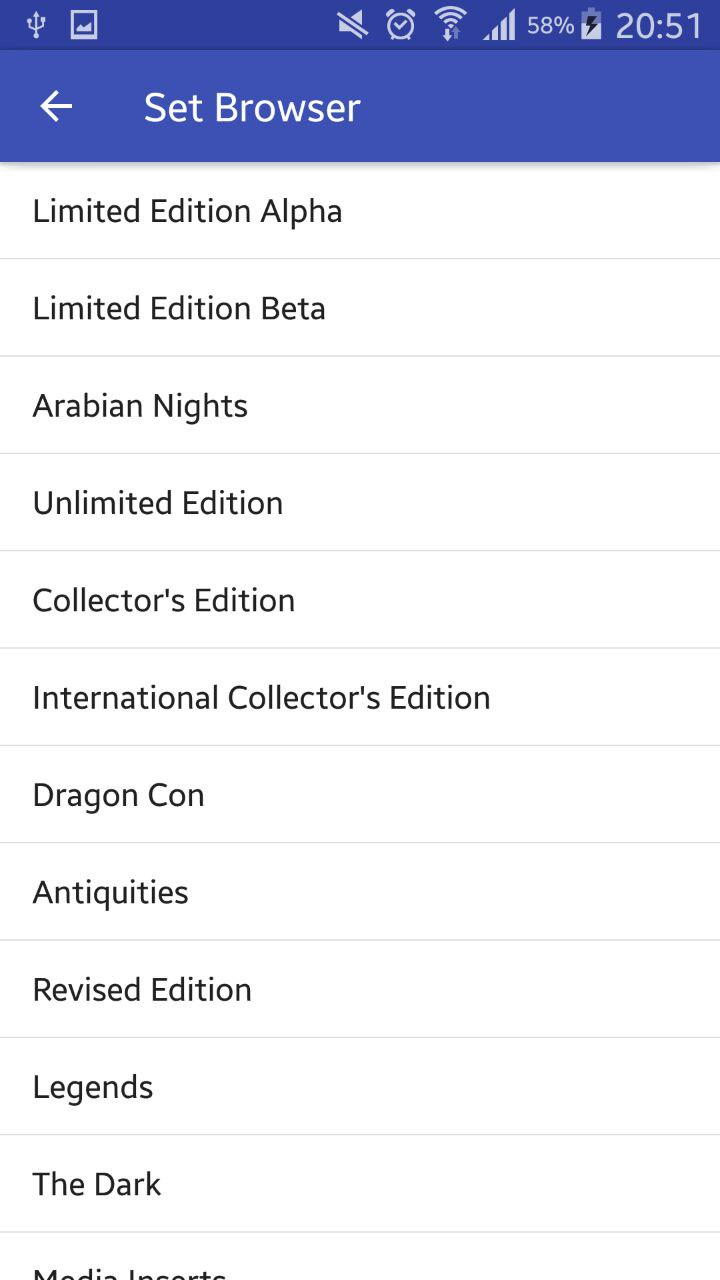
\includegraphics[width=0.3\textwidth]{setbrowser.jpg}
     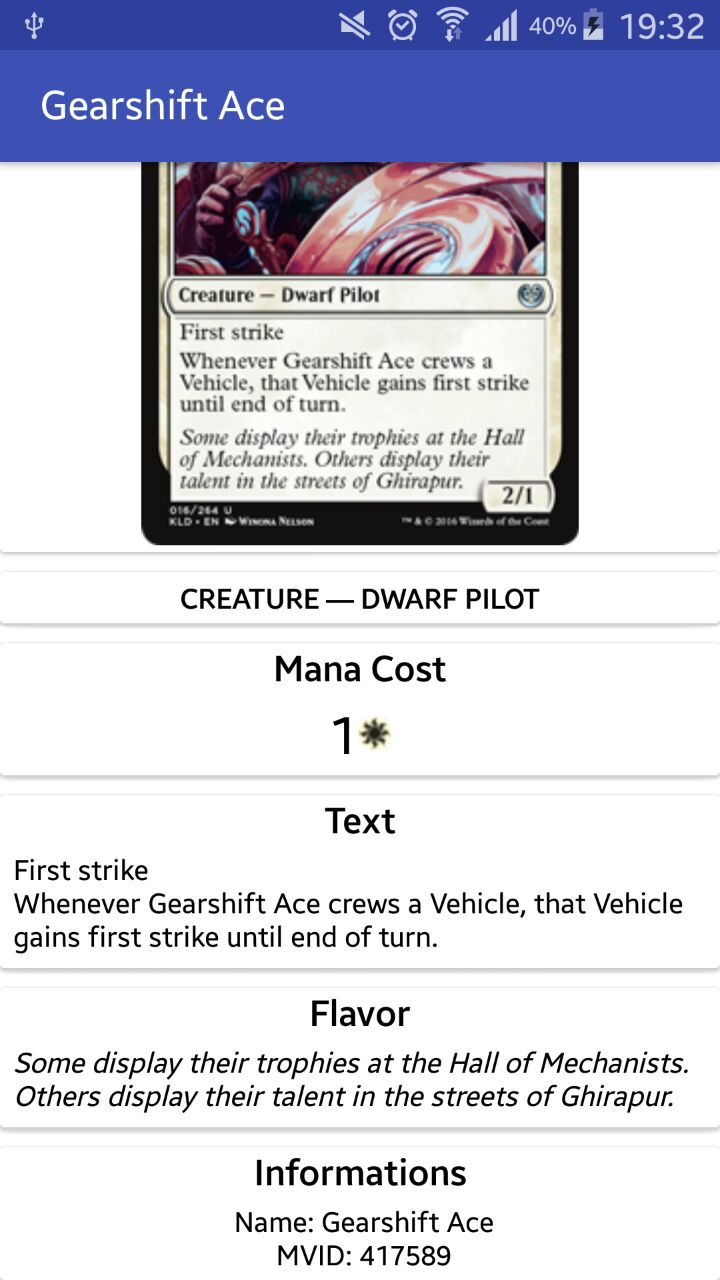
\includegraphics[width=0.3\textwidth]{cardview.jpg}
 \caption{Links: Der Set-Browser, Rechts: Die Karten-Ansicht \cite{Magiccard}}
 \label{fig:setbrowser}
\end{figure}

\subsection{Quick Learn}
"`Quick Learn"' startet eine Abfrage mit dem aktuellsten Set. In diesem Fall ist es Kaladesh. In der Mitte wird eine Karte vom Set gezeigt. Dabei ist der Text der Karte abgedeckt. Unterhalb der Karte befinden sich vier Schaltflächen mit verschiedenen Texten. Einer der Knöpfe enthält den Text der Karte. Drückt man die richtige Schaltfläche, wird kurz ein Haken auf die Karte projiziert, ansonsten ein Kreuz. Nach dieser Animation wird das Bild der Karte durch die nächste Karte im Set ersetzt. Die Schaltflächen ändern zudem ihren Text. Oben rechts befindet sich ein Menü-Sandwich. Bei dessen Betätigung sich ein Menü mit 3 Optionen öffnet: "`Query Lands"',"`Reverse query"' und "`Restart". Mit "`Query Lands"' kann man auswählen, ob die Länder auch abgefragt werden sollen. "`Reverse query" ändert den Abfragemodus. Im alternativen Modus ist der Name der Karte verdeckt. Unter der Karte befindet sich ein Textfeld, worin man den Namen der Karte eingeben soll. "`Restart" startet die ganze Abfrage neu (Abbildung \ref{fig:queryview}).

\begin{figure}[htbp]
 \centering
    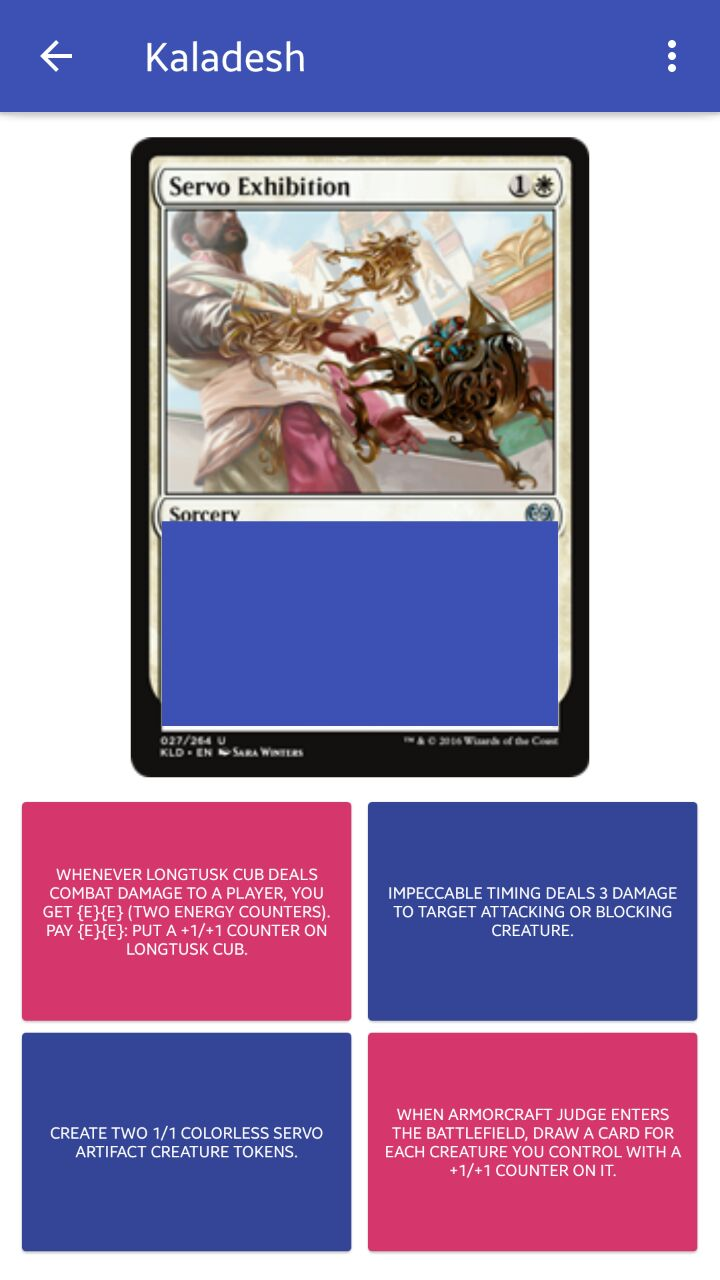
\includegraphics[width=0.3\textwidth]{query.jpg}
 \caption{Die Abfrage eines Sets \cite{Magiccard}}
 \label{fig:queryview}
\end{figure}

\subsection{Favorites}
Wechselt man auf den Reiter Favoriten, werden alle Karten, die als Favorit markiert wurden, in einer Liste angezeigt.

\subsection{Recently Learned}
"`Recently Learned"' zeigt die letzten 10 gelernten Sets in einer Liste an.

\subsection{Share}
Drückt man auf diese Schaltfläche, öffnet sich ein Menü. In diesem Menü kann man auswählen über welche App man den Link zu dieser App versenden möchte.
